\documentclass[conference]{IEEEtran}
\IEEEoverridecommandlockouts
\usepackage{cite}
\usepackage{amsmath,amssymb,amsfonts}
\usepackage{algorithmic}
\usepackage{graphicx}
\usepackage{textcomp}
\usepackage{xcolor}
\def\BibTeX{{\rm B\kern-.05em{\sc i\kern-.025em b}\kern-.08em
    T\kern-.1667em\lower.7ex\hbox{E}\kern-.125emX}}
\begin{document}

\title{SPARK-V: Small Power-Efficient Architecture for RISC-V}


\author{\IEEEauthorblockN{1\textsuperscript{st} Justin Lebeau}
\IEEEauthorblockA{\textit{Electrical and Computer Engineering} \\
\textit{Rice University}\\
Houston, Texas, United States \\
jhl6@rice.edu}
}

\maketitle

\begin{abstract}
Wearable biomedical devices require processors that balance performance with strict energy constraints, as battery life directly impacts usability and reliability in real world health monitoring. Current solutions often rely on proprietary low power processors, which can be expensive and lack flexibility for customization. Our project proposes an open-source alternative: developing and validating a low power RISC-V processor tailored for biomedical applications. We begin by validating an existing RISC-V core on an FPGA platform to demonstrate full functionality and suitability for wearable workloads. Building on this foundation, we target a 30\% reduction in system power through architectural and implementation-level optimizations. Ultimately, this project aims to produce a validated, energy efficient processor ready for tapeout, enabling more accessible and customizable solutions for biomedical wearables.
\end{abstract}

\begin{IEEEkeywords}
RISC-V, Low-Power Design
\end{IEEEkeywords}

\section{Introduction}
The design goal of this project is to create a processor for use in wearable biomedical devices. Since these devices are battery-powered, they require an architecture that is as low-energy as possible to maximize device usability and reliability.

While low-power processors currently exist, many of these are proprietary, which often makes them restrictive, expensive, or challenging to customize. To address this, the SPARK-V project proposes an open-source alternative using the RISC-V instruction set. The project begins by utilizing WALLY, an existing open-source RISC-V core from Harvey Mudd College, as a baseline [1].

\begin{figure}[htbp]
\centerline{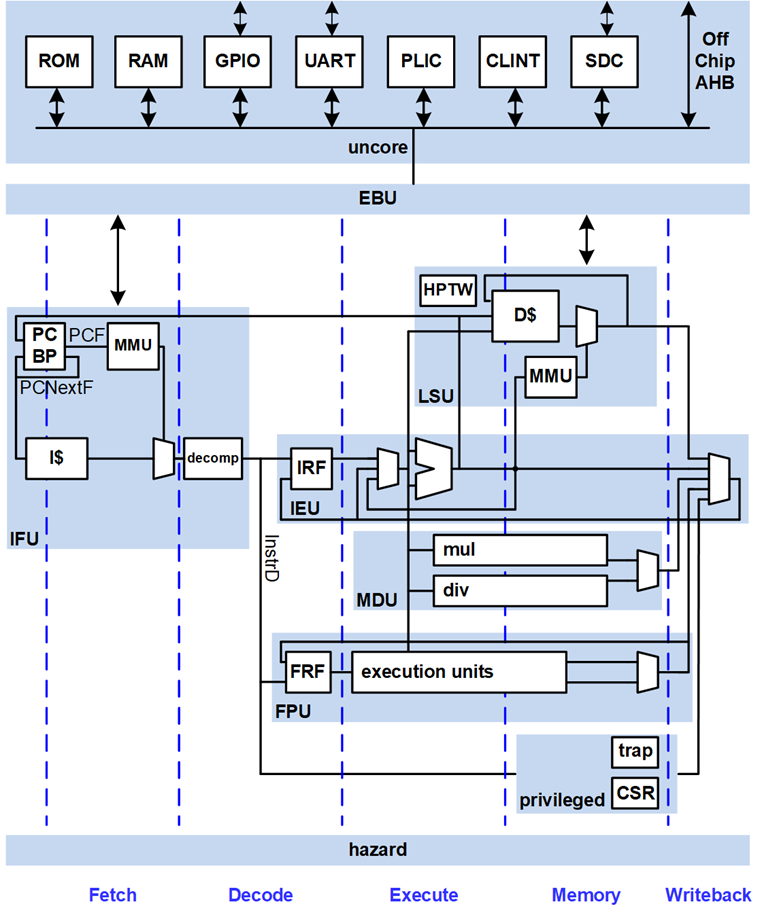
\includegraphics[width=0.9\linewidth]{WALLY_diagram.png}}
\caption{Block Diagram of the WALLY system [1]}
\label{fig}
\end{figure}

The primary goal is to achieve significant power efficiency, specifically targeting a 30\% reduction in system power. This will be accomplished through systematic architectural and implementation-level power optimizations, culminating in a validated, energy-efficient processor.

\section{Methods}

This project has been broken across two semesters, and thus I designed a set of goals for each semester. This semester, my first goal is to run Design Compiler for each potential configuration I identified last semester (RV32 IC, IMC, and IC\_Zmmul). Using Design Compiler allows each of these configurations to be synthesized, and for evaulation of their power, performance, and area. My second goal is to load each configuration onto an FPGA, and use the Embench test suite to test power usage of each configuration. Finally, I want to attempt to clock or input gate the multiplication and division unit of the processor to improve power usage.

\section{Results}

\subsection{Synthesis Using Design Compiler}

The initial phase of this project focused on utilizing Synopsys Design Compiler to synthesize three distinct configurations of the WALLY processor to establish an architectural baseline: RV32IC, RV32IC\_Zmmul, and RV32IMC. For this analysis, I used the Sky130 standard cell library. Although this 130 nm technology node is legacy hardware by modern standards, it provides a stable and consistent gate-level environment to evaluate the relative overhead of different RISC-V extensions, and is widely available. By maintaining a uniform timing constraint of a 25 MHz clock across all synthesis runs, I ensured that any fluctuations in the results were directly attributable to the architectural complexity of the extensions rather than variations in the physical synthesis flow.

The synthesis process yielded specific data points for total cell area, static leakage power, and dynamic switching power for each of the four configurations. These quantitative results now serve as the primary baseline against which the future clock-gating implementations in the multiplication and division unit will be evaluated for power efficiency improvements.

\begin{figure}[htbp]
\centerline{
\includegraphics[width=0.9\linewidth]{dc_results.png}}
\caption{Design Compiler Results}
\label{fig}
\end{figure}

Looking at these results, we can see some trends between the configurations. First, we can see that dynamic power is relatively consistent between the three configurations, with only a modest rise as complexity increases. However, static power shows a clearer increase with complexity. By including the MDU for multiplication only, the static power increases by 19\%, and when the MDU also does division, static power increases by 24\%. This correlates almost exactly to the area increase in these configurations, which makes sense as area and static power are directly correlated. Therefore, we can reduce static power by reducing processor complexity. While the dynamic power does not seem to change much, it is important to remember this is only an estimate, and more accurate data could be obtained by using real programs in simulation.

The timing reports also vary drastically between the configurations. As previously mentioned, all three designs were synthesized at a 25 MHz clock frequency, which corresponds to a 40 ns clock period. We can see the RV32IC configuration meets this with more than 17 ns to spare, meaning the clock frequency could be greatly increased for this configuration, or that lower power could be obtained by using a reduced voltage. However, the Zmmul configuration barely meets timing, and the IMC configuration has a small negative slack. This indicates that the multiplication and division instructions push timing to its limits, and make further critical path increases impossible at this frequency.

\subsection{Testing Embench on an FPGA}
In order to implement reduced configurations of WALLY on an FPGA, the workflow used on the Github required significant modification. As I did last semester, I am using the Arty A7 100T FPGA Board from Digilent as my FPGA platform. This board contains an AMD Artix-7 FPGA, as well as the needed connections for testing, including JTAG and UART support, as well as PMOD connectors that can be used to access an SD card [2].

\begin{figure}[htbp]
\centerline{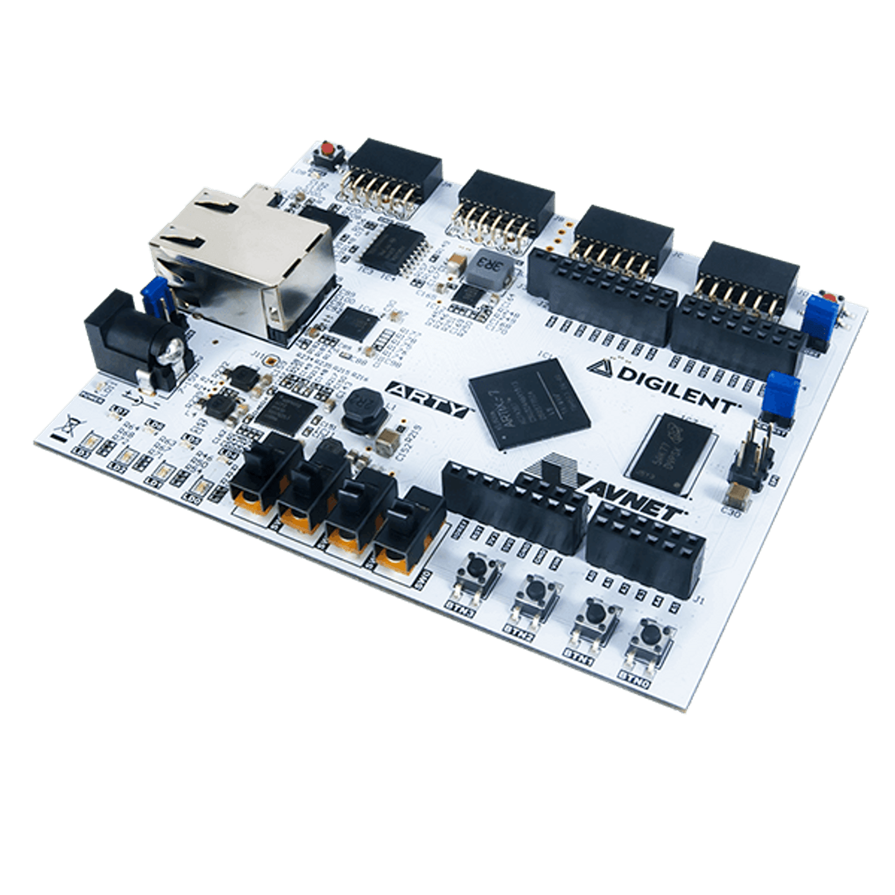
\includegraphics[width=0.9\linewidth]{Arty.png}}
\caption{The Arty A7 100-T FPGA Board [2]}
\label{fig}
\end{figure}

From last semester, I was able to boot linux on the FPGA by synthesizing the RV64gc configuration, and loading the necessary data onto a SD card. Upon power up, the processor would read a program in its bootrom that would instruct it to begin reading from the SD card, booting Linux.

However, for my testing purposes, I wanted to simplify the design to 32-bit configurations, as well as store the program data directly in the processor rather than on external memory.

To start, I modified the Makefile and TCL scrips that invoked Vivado for the FPGA build. I had to make several changes to allow 32 bit compilation, as well as create new configration files to allow for reduced extension inclusions. Then, I overwrote the bootrom loading process to allow the processor to store my desired program in bootrom rather than the SD card startup code. This has allowed me to add test programs directly into the processor ROM.

I have so far been able to load some small test programs into memory, and generate a FPGA bitstream with them. However, I still need to be able to compile the actual Embench programs, as these are somewhat more complex.

To start, I tested one Embench program, crc32, in simulation using Questa. This program computes a cyclic redundancy check (CRC), and its main function and Questa results can be seen in figure 4.

\begin{figure}[htbp]
\centerline{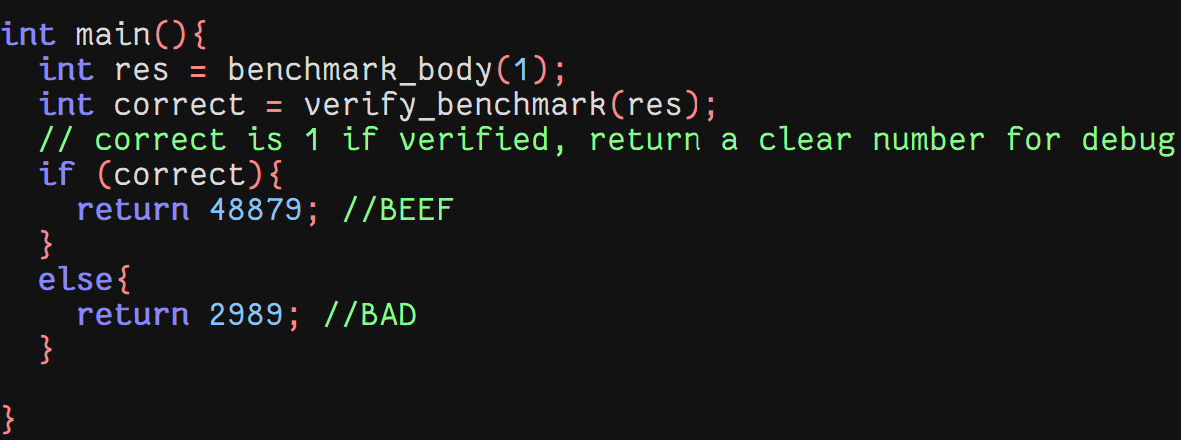
\includegraphics[width=0.9\linewidth]{crc_benchmark.png}}
\centerline{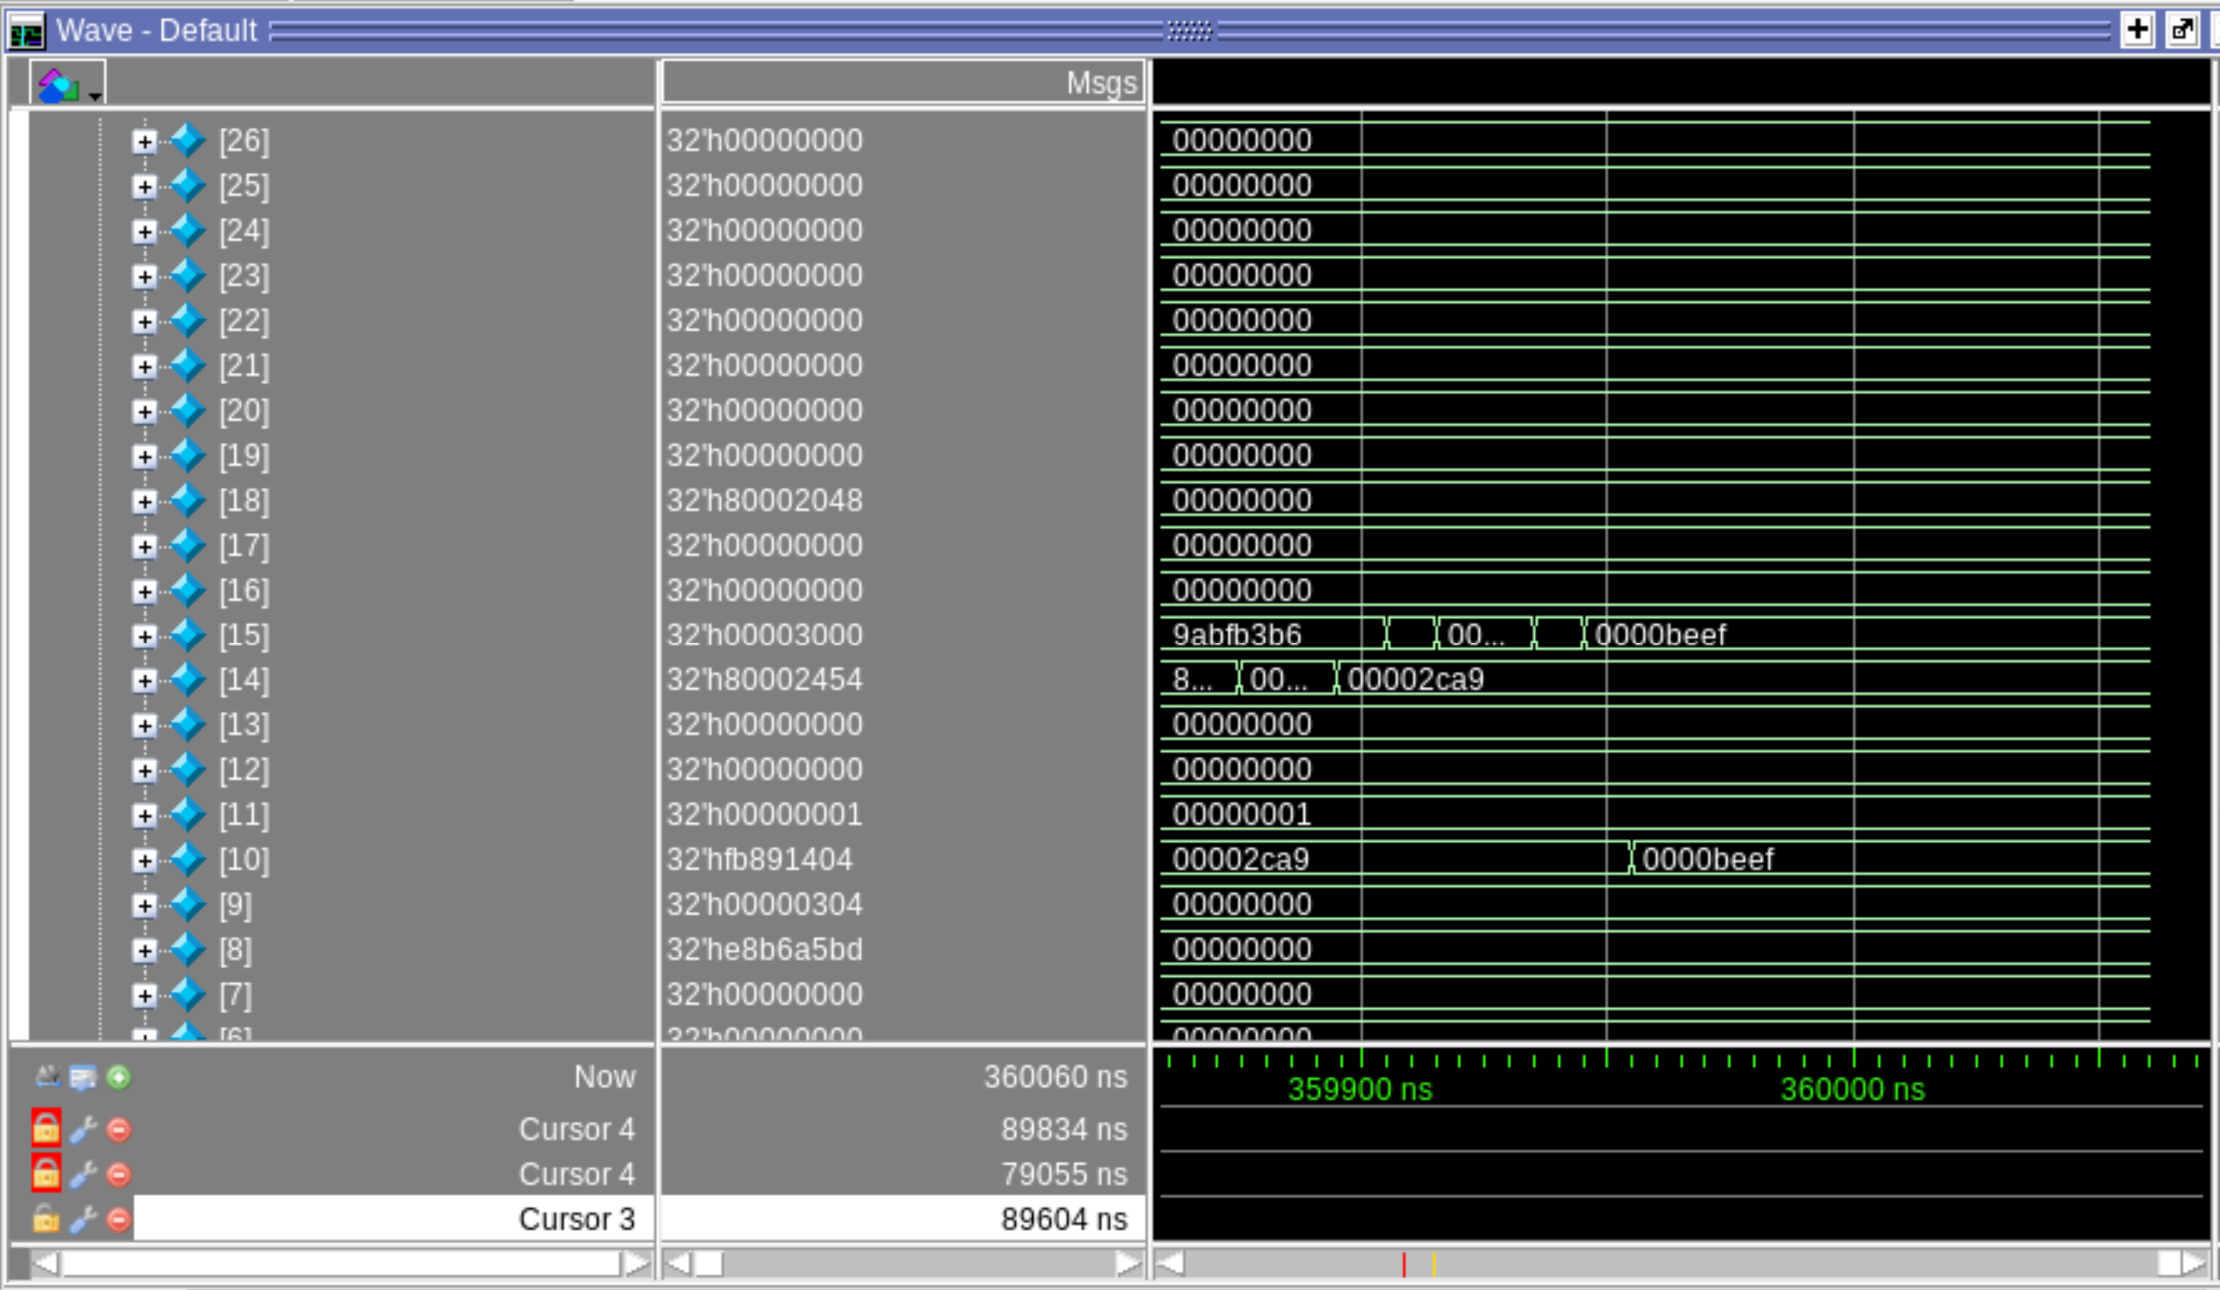
\includegraphics[width=0.9\linewidth]{crc_result.png}}
\caption{The crc32 main function (top), and Questa results showing final register values (bottom),}
\label{fig}
\end{figure}

The main function calls the benchmark\_body function, which computes the CRC, then calls a function to verify that the final value produced is the expected value. If so, main returns the value 0xbeef into the return register, and if not it returns 0xbad. These values were chosen to aid in debugging. From the Questa waveform, it can be seen that the processor has the correct value in its return register x10 at the end of program execution, indicating the benchmark simulates correctly.

While I have been able to load this program into the FPGA boot ROM, I do not yet have a way to get information back out of the FPGA to measure power and performance. This is one of my focuses for the remainder of the semester.


\subsection{MDU Clock Gating}

Clock gating is a powerful technique to reduce power usage, but its effectiveness varies based on the frequency that a given unit is in use. After discussion with various members of the WALLY project, we agreed that for an integer machine, the majority of functional units are in use at a high enough frequency that the work required to implement fine-grain clock gating would not be worth the effort, and could contradict standard design processes. However, one unit that is often idle is the actual multiplication and division unit (MDU).

I plan on implementing either clock or input gating to the MDU to help reduce power consumption. I have attempted this, but ran into issues, and will retry during the remaining part of the semester.

\subsection{Peripherals}
WALLY contains a number of peripherals in the "uncore" module. These include ROM, RAM, timers, GPIO, and communication over UART. While the design of the core has been specified above, additional work will be needed to decide which uncore components will be used, and what settings will be applied to them.

Currently, it makes sense to include all of these peripherals to some extent. Program ROM and RAM are fundamental for any standalone system, and the inclusion of PLIC and CLINT enables timer-driven and interrupt-driven execution, both of which are standard requirements for embedded workloads. UART, SDC, and GPIO interfaces also provide practical pathways for off-chip communication, data transfer, and basic system control, making them useful for both development and deployment. In practice, the exact set of peripherals will depend on system constraints. For example, GPIO is flexible and broadly applicable, but the number of exposed pins may need to be reduced if the final processor package has limited I/O availability. Careful selection and scaling of these peripherals will help ensure functionality without exceeding physical or architectural constraints.

\section{Discussion}
My work this semester has helped to identify key areas for future work on the SPARK-V processor. Synthesis results using the Sky130 logic library highlight a direct correlation between architectural complexity and power consumption. The transition from a base RV32IC configuration to the RV32IMC, which includes multiplication and division, resulted in a 24\% increase in static power. This increase is almost entirely driven by the expanded silicon area required for the multiplication and division unit. Therefore, a low-power design should focus on optimizing as simple a processor as will be useful.

My two primary targets for the remainder of the semester FPGA benchmarking and gating the MDU to improve power. My main roadblock in the FPGA testing is my inability to extract information from the processor core. The UART and GPIO modules should be able to transmit information, but I need to figure out how to connect these properly and program the core to send this information out. For the MDU, making the RTL change should be possible without too much effort, but measuring a power change may be slightly more difficult. Although measuring fine-grained power fluctuations on an FPGA presents a challenge, these optimizations are essential for ensuring the processor is ready for a power-efficient tapeout.



\section*{Acknowledgment}

I would like to thank Dr. Ray Simar for his support on this project, as well as Dr. James Stine and Jacob Pease from Oklahoma State University for their continued guidance. I would also like to thank David Harris and Sarah Harris for granting pre-publication access to their textbook covering the WALLY design which has helped in understanding the processor. Additionally, thanks to the Rice Electrical and Computer Engineering Department for funding this project.

\section*{CRediT Author Statement}
\textbf{Justin Lebeau:}
Conceptualization, Investigation, Methodology, Software, Validation, Writing

\begin{thebibliography}{00}
\bibitem{b1} https://github.com/openhwgroup/cvw
\bibitem{b2} https://digilent.com/shop/arty-a7-100t-artix-7-fpga-development-board/

\end{thebibliography}

\end{document}
